% stuff

\documentclass[prl,twocolumn,showpacs,superscriptaddress,preprintnumbers,floatfix]{revtex4-1}

% ******************************************************************************
%%% Imports and configuration

\usepackage{etex}                        %
\usepackage{ifpdf}                       %
\usepackage[final,pagebackref]{hyperref} %
\usepackage{graphicx}                    %
\usepackage{dcolumn}                     %
\usepackage{url}                         %
\usepackage{amsmath}                     %
\usepackage{amscd}                       %
\usepackage{amsfonts}                    %
\usepackage{amssymb}                     %
\usepackage{amsthm}                      %
\usepackage{bm}                          %
\usepackage{bbm}                         %
\usepackage{verbatim}                    %
\usepackage{stmaryrd}                    %
\usepackage{xcolor}                      %
\usepackage{setspace}                    %
\usepackage{xspace}                      % Let macros play nice with spaces
\usepackage{nicefrac}                    % Pretty fractions
\usepackage{cleveref}                    % Automatically label references
\usepackage{booktabs}                    % Nicer tables
\usepackage[caption=false]{subfig}       % Subfigures

%% Various TikZ related imports
\usepackage{tikz}
\usetikzlibrary{arrows}
\usetikzlibrary{automata}
\usetikzlibrary{calc}
\usetikzlibrary{decorations.pathreplacing}
\usetikzlibrary{external}
\usetikzlibrary{intersections}
\usetikzlibrary{patterns}
\usetikzlibrary{plotmarks}
\usetikzlibrary{positioning}
\usetikzlibrary{through}
%\tikzexternalize
\tikzsetexternalprefix{images/}
\tikzstyle{vaucanson}=[
  %node distance=1.25cm,
  node distance=3cm,
  bend angle=15,
  auto,
  % For some reason, the loop direction cannot be overwritten if we set the
  % style for "every loop" to be "->".  Curiously, this doesn't seem to be
  % an issue for "every edge".
  every loop/.style={},
  every edge/.style={->,draw=black,line width=1.2,>=latex,shorten <=1pt, shorten >=1pt},
  every state/.style={draw=black,line width=2,font=\large},
  loop right/.style={right,out=22,in=-22,loop},
  loop above/.style={above,out=112,in=68,loop},
  loop left/.style={left,out=202,in=158,loop},
  loop below/.style={below,out=292,in=248,loop},
  loop above right/.style={right,out=67,in=23,loop},
  loop above left/.style={left,out=157,in=113,loop},
  loop below left/.style={left,out=247,in=203,loop},
  loop below right/.style={right,out=337,in=293,loop},
  binode/.style={minimum size=1cm,inner sep=0pt},
]

\tikzset{
  mystate/.style={circle,draw,fill=black}
}

%%% Command for bicausal nodes. This only supports relative positioning.
%%% Use as: \binode[state][red,blue] (AC) [left=of someNode] {$\A:\:C$};
\makeatletter
\newcommand{\binode}[1][state]{%
  \@ifnextchar[{\binode@i[{#1}]}{\binode@i[{#1}][{yellow},{gray!70}]}%
}
\def\binode@i[#1][#2,#3]{%
  \@ifnextchar({\binode@ii[{#1}][{#2},{#3}]}{\binode@ii[{#1}][{#2},{#3}]({})}%
}
\def\binode@ii[#1][#2,#3](#4){%
  \@ifnextchar[{\binode@iii[{#1}][{#2},{#3}]({#4})}{\binode@iii[{#1}][{#2},{#3}]({#4})[{}]}%
}
\def\binode@iii[#1][#2,#3](#4)[#5]#6{%

  \node[#1,binode] (#4) [#5] {#6};
  \node[yshift=-10pt] (#4SS) at (#4.270) {};
  \node[xshift=-10pt] (#4WW) at (#4.180) {};
  \node[xshift=-10pt] (#4NN) at (#4.180) {};
  \node[xshift=-10pt,yshift=10pt] (#4NW) at (#4.135) {};
  % forward shading
  \begin{scope}
    \path[clip] (#4.255) -- +(-.8cm,0cm) -- +(-.8cm,1cm) -- (#4.75) -- cycle;
    \node[#1,fill=#2,binode] (#4f) [#5] {#6};
  \end{scope}
  % reverse shading
  \begin{scope}
    \path[clip] (#4.75) -- +(.8cm,0cm) -- +(.8cm,-1cm) -- (#4.255) -- cycle;
%    ++(0cm,-.2cm) -- ++(.8cm,0cm)  -- ++(0cm,1cm) -- (#4.75) -- cycle;
    \node[#1,fill=#3,binode] (#4r) [#5] {#6};
  \end{scope}
  \node {} % semicolon purposefully omitted. this is a dummy call
}
\makeatother

\providecommand{\Symbol}[1]{\textcolor{blue}{#1}}
\providecommand{\Edge}[2]{\Symbol{#1}\!:\!#2}
\providecommand{\TEdge}[3]{\Symbol{#1}|\Symbol{#2}\!:\!#3}

\definecolor{FCSA}{RGB}{141,211,199}
\definecolor{FCSB}{RGB}{255,255,179}
\definecolor{RCSC}{RGB}{185,138,196}
\definecolor{RCSD}{RGB}{231,143,111}
\definecolor{RCSE}{RGB}{128,177,211}


\usepackage{pgfplots}
\pgfplotsset{compat=newest}

% Useful TikZ code stolen from http://tex.stackexchange.com/a/71596/66712
\tikzset{
  anticlockwise arc centered at/.style={
    to path={
      let \p1=(\tikztostart), \p2=(\tikztotarget), \p3=(#1) in
      \pgfextra{
        \pgfmathsetmacro{\anglestart}{atan2(\x1-\x3,\y1-\y3)}
        \pgfmathsetmacro{\angletarget}{atan2(\x2-\x3,\y2-\y3)}
        \pgfmathsetmacro{\angletarget}%
        {\angletarget < \anglestart ? \angletarget+360 : \angletarget}
        \pgfmathsetmacro{\radius}{veclen(\x1-\x3,\y1-\y3)}
      }
      arc(\anglestart:\angletarget:\radius pt) -- (\tikztotarget)
    },
  },
  clockwise arc centered at/.style={
    to path={
      let \p1=(\tikztostart), \p2=(\tikztotarget), \p3=(#1) in
      \pgfextra{
        \pgfmathsetmacro{\anglestart}{atan2(\x1-\x3,\y1-\y3)}
        \pgfmathsetmacro{\angletarget}{atan2(\x2-\x3,\y2-\y3)}
        \pgfmathsetmacro{\angletarget}%
        {\angletarget > \anglestart ? \angletarget - 360 : \angletarget}
        \pgfmathsetmacro{\radius}{veclen(\x1-\x3,\y1-\y3)}
      }
      arc(\anglestart:\angletarget:\radius pt)  -- (\tikztotarget)
    },
  },
}

%% Used for code samples
\usepackage{listings}
\lstdefinestyle{mypython}{
language=Python,                        % Code langugage
basicstyle=\small\ttfamily,             % Code font, Examples: \footnotesize, \ttfamily
keywordstyle=\color{green!50!black},    % Keywords font ('*' = uppercase)
commentstyle=\color{gray},              % Comments font
numbers=left,                           % Line nums position
numberstyle=\tiny,                      % Line-numbers fonts
stepnumber=1,                           % Step between two line-numbers
numbersep=5pt,                          % How far are line-numbers from code
backgroundcolor=\color{gray!10},        % Choose background color
frame=none,                             % A frame around the code
tabsize=2,                              % Default tab size
captionpos=b,                           % Caption-position = bottom
breaklines=true,                        % Automatic line breaking?
breakatwhitespace=false,                % Automatic breaks only at whitespace?
showspaces=false,                       % Dont make spaces visible
showtabs=false,                         % Dont make tabls visible
morekeywords={as},                      % Additional keywords
}

%% Finally, computational mechanics macros.
\input{cmechabbrev}

%% Uncomment to list package versions
%\listfiles

\setlength{\parindent}{0pt}

\newcommand{\alert}[1]{\textbf{\textcolor{red}{#1}}}


%% Various theorem styles
\theoremstyle{plain}    \newtheorem{Lem}{Lemma}
\theoremstyle{plain}    \newtheorem*{ProLem}{Proof}
\theoremstyle{plain}    \newtheorem{Cor}{Corollary}
\theoremstyle{plain}    \newtheorem*{ProCor}{Proof}
\theoremstyle{plain}    \newtheorem{The}{Theorem}
\theoremstyle{plain}    \newtheorem*{ProThe}{Proof}
\theoremstyle{plain}    \newtheorem{Prop}{Proposition}
\theoremstyle{plain}    \newtheorem*{ProProp}{Proof}
\theoremstyle{plain}    \newtheorem*{Conj}{Conjecture}
\theoremstyle{plain}    \newtheorem*{Rem}{Remark}
\theoremstyle{plain}    \newtheorem{Def}{Definition}
\theoremstyle{plain}    \newtheorem*{Not}{Notation}

% ******************************************************************************
% Set up pdf stuff

\newcommand{\arxiv}[1]{\href{http://arxiv.org/abs/#1}{\texttt{arXiv}:#1}}
 % SFI working papers do not have friendly URLs.
\newcommand{\sfiwp}[1]{Santa Fe Institute Working Paper #1}

\begin{document}

\def\ourTitle{%
  Title goes here.
}

\def\ourAbstract{%
  Abstract goes here.
}

\def\ourKeywords{%
 stochastic process, hidden Markov model,
  \texorpdfstring{\eM}{epsilon-machine}, causal states, mutual information.
}

\hypersetup{
  pdfauthor={James P. Crutchfield},
  pdftitle={\ourTitle},
  pdfsubject={\ourAbstract},
  pdfkeywords={\ourKeywords},
  pdfproducer={},
  pdfcreator={}
}

\author{Ryan G. James}
\email{rgjames@ucdavis.edu}
\affiliation{Complexity Sciences Center and Physics Department,
University of California at Davis, One Shields Avenue, Davis, CA 95616}

% \author{John Mahoney}
% \email{jmahony@ucdavis.edu}
% \affiliation{Complexity Sciences Center and Physics Department,
% University of California at Davis, One Shields Avenue, Davis, CA 95616}

\author{James P. Crutchfield}
\email{chaos@ucdavis.edu}
\affiliation{Complexity Sciences Center and Physics Department,
University of California at Davis, One Shields Avenue, Davis, CA 95616}
\affiliation{Santa Fe Institute, 1399 Hyde Park Road, Santa Fe, NM 87501}

\date{\today}
\bibliographystyle{unsrt}


% ******************************************************************************
% TikZ graphics setup

\colorlet {past_color}    {red}
\colorlet {pres_color}    {blue}
\colorlet {futu_color}    {black!30!green}

\colorlet {temp_color_1}  {red!50!blue}
\colorlet {temp_color_2}  {red!50!green}
\colorlet {temp_color_3}  {blue!50!green}

\colorlet {hmu_color}     {blue!67!green}
\colorlet {rhomu_color}   {temp_color_1!80!blue}
\colorlet {rmu_color}     {blue}
\colorlet {bmu_1_color}   {temp_color_1}
\colorlet {bmu_2_color}   {temp_color_3}
\colorlet {qmu_color}     {temp_color_1!67!green}
\colorlet {wmu_color}     {temp_color_2!57!blue}
\colorlet {sigmamu_color} {temp_color_2}

\def \idiagramsetup {
  \def \radius {1.5}
  \def \delt {2}
  \def \diff {0.04}

  \coordinate (A) at (0, 0);
  \coordinate (B) at (240:\delt);
  \coordinate (C) at (-60:\delt);
  \coordinate (D) at ($ (C) ! 0.33 ! 30:(A) $);
  \coordinate (T) at ($ (A) ! \radius ! (0, 1) $);
  \coordinate (center) at (barycentric cs:A=1/3,B=1/3,C=1/3);

  \path [ultra thick, name path=present] (A) circle (\radius);
  \path [ultra thick, name path=fcsz]    (B) circle (\radius);
  \path [ultra thick, name path=rcso]    (C) circle (\radius);

  \path [name intersections={of=present and rcso, by={i1, i2}}];
  \path [name intersections={of=fcsz and rcso, by={i3, i4}}];
  \path [name intersections={of=fcsz and present, by={i5, i6}}];

  \path [ultra thick, name path=fcso, line join=round, green] ($ (i2) ! \diff ! (A) $) to
        [anticlockwise arc centered at=D] ($ (i4) ! \diff ! (B) $) to
        [anticlockwise arc centered at=B] ($ (i5) ! \diff ! (B) $) to
        [clockwise arc centered at=i5] ($ (i5) ! \diff ! (A) $) to
        [anticlockwise arc centered at=A] ($ (i2) ! \diff ! (A) $);

  \path [name intersections={of=fcso and fcsz, by={i7, i8}}];
  \path [name intersections={of=fcso and present, by={i9, i10}}];
}

\def \present { (A) circle (\radius) }
\def \fcsz { (B) circle (\radius) }
\def \fcso {
  [line join=round] ($ (i2) ! \diff ! (A) $) to
  [anticlockwise arc centered at=D] ($ (i4) ! \diff ! (B) $) to
  [anticlockwise arc centered at=B] ($ (i5) ! \diff ! (B) $) to
  [clockwise arc centered at=i5] ($ (i5) ! \diff ! (A) $) to
  [anticlockwise arc centered at=A] ($ (i2) ! \diff ! (A) $)
}
\def \rcso { (C) circle (\radius) }

\def \labelpresent { \node at ($ (center) ! 2.6 ! (A) $) {\H{\textcolor{pres_color}{\Present}}} }
\def \labelfcsz { \node at ($ (center) ! 2.85 ! (B) $) {\H{\textcolor{past_color}{\FCS_0}}} }
\def \labelrcso { \node at ($ (center) ! 2.85 ! (C) $) {\H{\textcolor{futu_color}{\RCS_1}}} }
\def \labelfcso { \node at ($ (center) ! 1.5 ! (i2) $) {\H{\FCS_1}} }

\def \locationa { ($ (i3) ! 0.5 ! (T) $) }
\def \locationb { ($ (i3) ! 0.15 ! (T) $) }
\def \locationc { (barycentric cs:i6=5/12,i7=7/24,i9=7/24) }
\def \locationd { (barycentric cs:i1=1/5,i3=1/5,i7=3/10,i9=3/10) }
\def \locatione { (barycentric cs:i1=1/3,i3=1/3,i5=1/3) }
\def \locationf { (barycentric cs:i2=5/12,i3=7/24,i5=7/24) }
\def \locationg { ($ (i1) ! 0.55 ! (B) $) }
\def \locationh { (barycentric cs:i1=7/24,i4=5/12,i5=7/24) }
\def \locationi { ($ (i1) ! 2 ! (B) $) }
\def \locationj { ($ (i5) ! 1.6 ! (C) $) }
\def \locationk { (barycentric cs:i5=5/12,i7=7/24,i9=7/24) }
\def \locationl { (barycentric cs:i2=1/2,i5=1/5,i7=3/10) }
\def \locationm { (barycentric cs:i4=1/2,i5=1/5,i9=3/10) }
\def \locationn { (barycentric cs:i1=7/24,i3=7/24,i6=5/12) }
\def \locationo { ($ (i1) ! 1.6 ! (B) $) }


% ******************************************************************************
% The paper content

\title{\ourTitle}

\begin{abstract}

\ourAbstract

\vspace{0.1in}
\noindent
{\bf Keywords}: \ourKeywords

\end{abstract}

\pacs{
05.45.-a  %  Nonlinear dynamics and nonlinear dynamical systems
89.75.Kd  %  Complex Systems: Patterns
89.70.+c  %  Information science
05.45.Tp  %  Time series analysis
%02.50.Ey  %  Stochastic processes
%02.50.-r  %  Probability theory, stochastic processes, and statistics
%02.50.Ga  %  Markov processes
%05.20.-y  %  Classical statistical mechanics
}

\preprint{\sfiwp{13-11-XXX}}
\preprint{\arxiv{1312.XXXX}}

\title{\ourTitle}
\date{\today}
\maketitle
\tableofcontents

\setstretch{1.1}



\section{Introduction}
\label{sec:introduction}

This is an introduction. See \cref{fig:even_process} for more information.

\begin{figure}
  \centering
  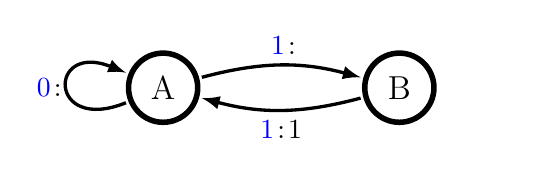
\begin{tikzpicture}[style=vaucanson,
                      bend angle=15,
                      scale=1,
                      every node/.style={transform shape}]
    \node [state] (A)              {A};
    \node [state] (B) [right of=A] {B};

    \path (A) edge [loop left] node {$\Edge{0}{\half}$} (A)
          (A) edge [bend left] node {$\Edge{1}{\half}$} (B)
          (B) edge [bend left] node {$\Edge{1}{1}$}     (A);
    % added for symmetry
    \path (B) edge [loop right, draw=none] node {} (B);
  \end{tikzpicture}
  \label{fig:even_process}
\end{figure}

\section*{Acknowledgments}
\label{sec:acknowledgments}

We thank people for things.

\bibliography{chaos,ref}

\cleardoublepage

\appendix

\section{Appendix A}
\label{sec:appendix_a}

This is an appendix, if it is needed.

\end{document}
